\section{Manual}
\label{sec:manual}
\subsection{Systemvorraussetzungen \& Kompilation}
Das Framework nutzt verschiedene Bibliotheken zum Testen, Generieren von Vektorbildern, Datenbankzugriff und zur Parsierung von Kommandozeilenparametern. Wir nutzen Maven2 als \emph{build tool}, um diese Abhängigkeiten automatisiert aufzulösen. Die Kompilation wurde von uns ausschließlich unter GNU/Linux-Systemen getestet, jedoch sollte die Portierung nach Microsoft Windows leicht möglich sein. Vorraussetzungen für eine erfolgreiche Kompilation sind (in Klammern die Namen der Pakete bei Debian/Ubuntu-Systemen mit erfolgreich getesteten Versionsnummern):
\begin{itemize}
	\item Java 1.6 Development Kit (\texttt{openjdk-6-jdk}, Version \enquote{6b18-1.8.7-2~squeeze1})
	\item Maven 2 (\texttt{maven2}, Version 2.2.1-5)
\end{itemize}

Weiterführende Informationen zur Kompilierung des Projekts finden sich in der beiliegenden \texttt{README}-Datei.

\subsection{Grafische Oberfläche}
Die Oberfläche ist dazu da Polygone zu generieren, den Shortest Path zu berechnen und diesen darzustellen.\\
\begin{center}
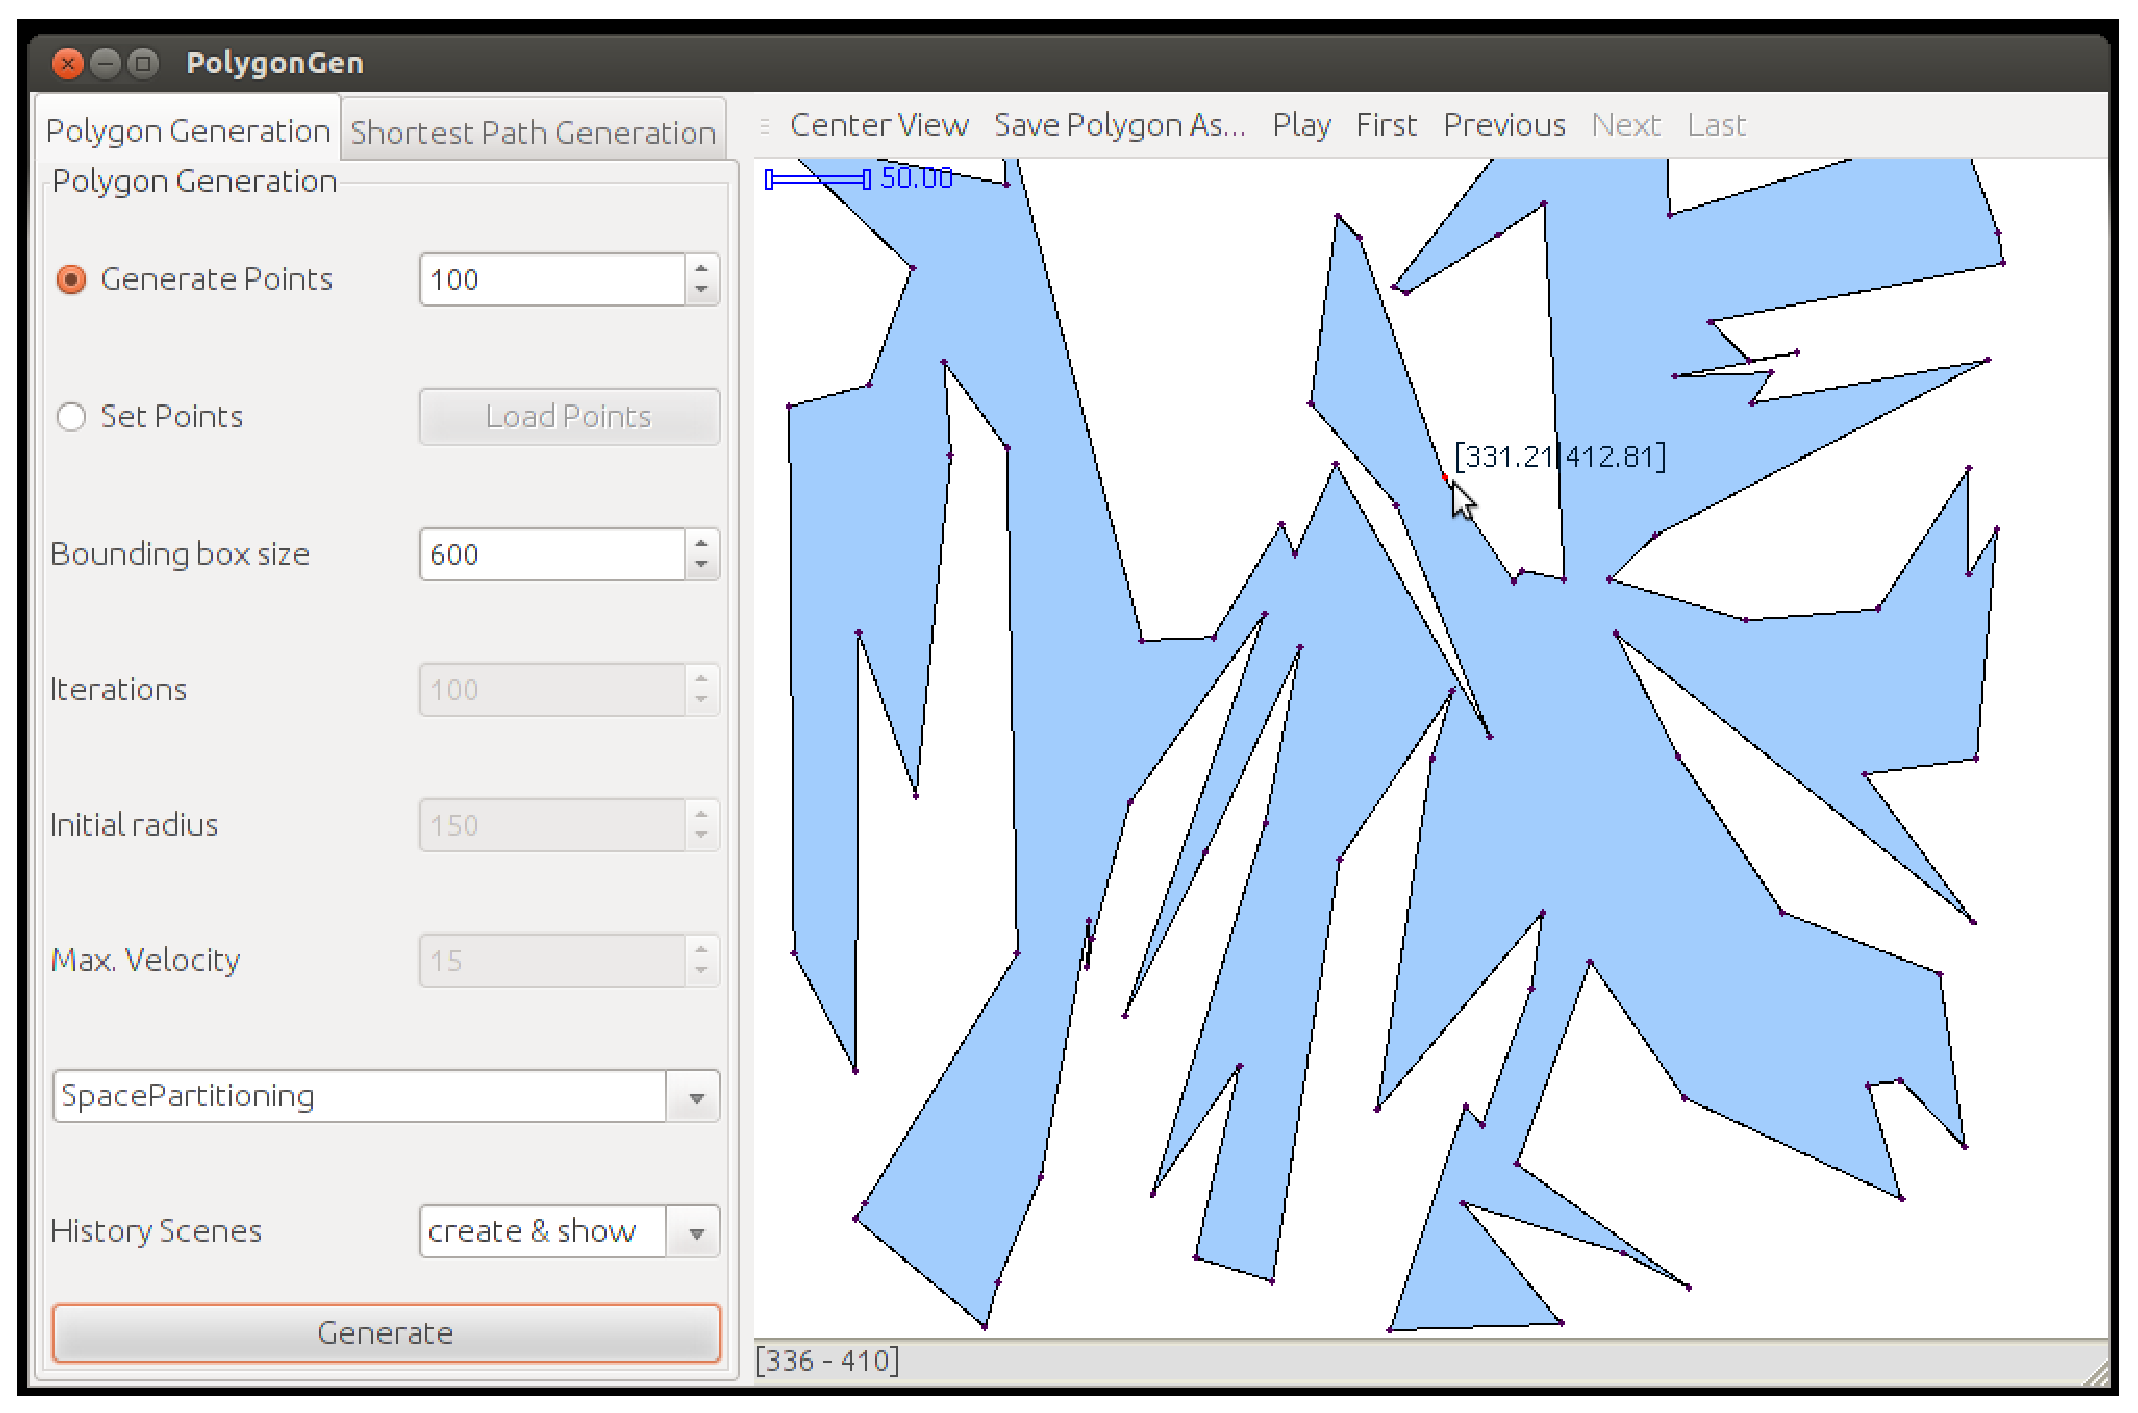
\includegraphics[width=0.7\textwidth]{img/GUI.eps}
\end{center}

\subsubsection{Funktionen}
\begin{itemize}
	\item Generierung von Polygonen
	\item Visualisierung der Polygon-Algorithmen
	\item Manuelle Auswahl der Punktmenge eines Polygons
	\item Zoomen und Bewegen
	\item Anzeigen der Werte einzelner Polygone
	\item Berechnung des Shortest-Path
	\item Speichern des Polygons
\end{itemize}

\subsection{Kommandozeile}
Mit der Kommandozeile ist es möglich mehrere Polygone und deren Statistiken gleichzeitig zu erzeugen und diese in eine Ausgabedatei zu schreiben. Zusätzlich ist es möglich die Anzahl der Threads zu bestimmen für optimales paralleles Berechnen. Damit ist es möglich viele verschiedene Polygone mit den gleichen Parametern zu erzeugen. Die Parameter werden im \enquote{GNU-Stil} angegeben.\\
Um die Usage-Hilfe zu bekommen ruft man das Programm mit dem Parameter --help oder --usage auf. Listing~\ref{listing_usage} zeigt einen gekürzten Ausschnitt aus der Usage. Alle weiteren Parameter sind in der Usage näher erläutert.

\begin{code}[caption={Usage der Kommandozeile},label=listing_usage]
usage: run.sh [--algorithm <Algorithm>] [--boundingbox <boundingbox>]
       [--database <Database file>] [--help] [--number <Number of
       polygons>] [--output <Output path>] [--points <Number of points>]
       [--radius <circle radius>] [--runs <number of runs>] [--threads
       <Number of threads>] [--usage] [--velocity <velocity>]
-
Use with no arguments to show GUI, use --output and/or --database to start
batch-mode.
-
    --algorithm <Algorithm>         The algorithm to execute, specified by
                                    ID (Default: 0). Available algorithms:
                                    [0] SpacePartitioning
                                    [1] Permute & Reject
                                    [2] 2-Opt moves
                                    [3] RandomPolygonAlgorithm
                                    [4] Incremental Construction &
                                    Backtracking
                                    [5] ConvexHull
                                    [6] Velocity Virmani
                                    [7] SteadyGrowth
                                    [8] TwoPeasants

[...]
\end{code}

\begin{code}[caption={Beispiel-Ausführung},label=listing_usage_example]
\$ run.sh --algorithm 0 --number 10 --points 25 --output out/polygon
\end{code}

Das Beispiel-Kommando in Listing~\ref{listing_usage_example} führt zur Generierung von 10 Polygonen mit je 25 Punkten mit Hilfe des \emph{Space Partitioning}-Algorithmus. Die erzeugten Polygone werden im Verzeichnis \texttt{out} unter dem Namen \texttt{polygon-01}, \texttt{polygon-02}, usw. gespeichert.
